\documentclass{article}

\usepackage[utf8]{inputenc}
\usepackage[spanish,mexico]{babel}
\usepackage{parskip} 
\usepackage[margin=2.5cm]{geometry}
\usepackage{graphicx}
\usepackage{float}
\usepackage{amsmath}
\usepackage{booktabs}
\usepackage{hyperref}
\usepackage{mathpazo}
\usepackage{fancyhdr}
\usepackage{enumitem} 

\pagestyle{fancy}
\fancyhf{}
\fancyfoot[C]{\thepage}

\begin{document}
\thispagestyle{empty}

\begin{minipage}{0.22\linewidth}
    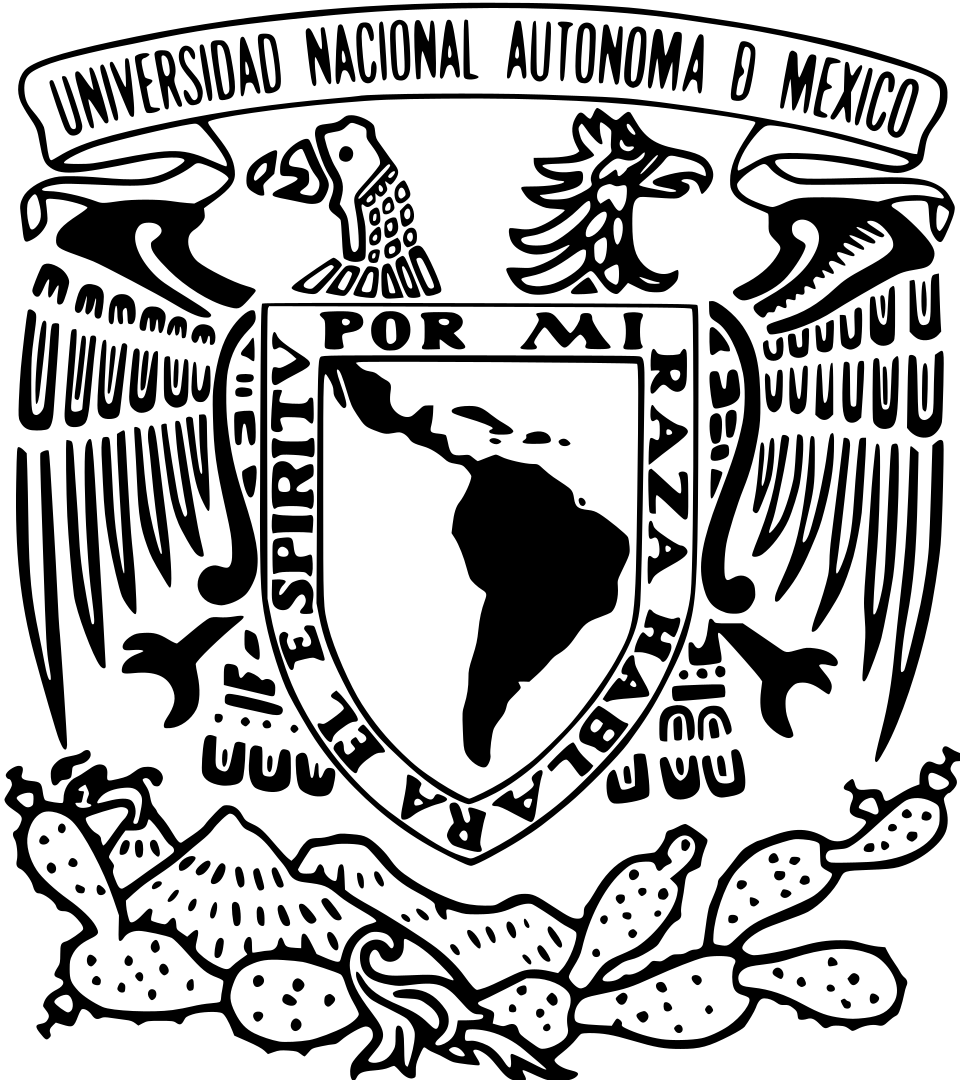
\includegraphics[scale=0.08]{unam.png} 
\end{minipage}
\begin{minipage}[c]{0.53\linewidth}
    \begin{center}
        {\Large UNIVERSIDAD NACIONAL AUTÓNOMA DE MÉXICO \vspace{0.80cm}}\\
        {\Large Facultad de Ingeniería \vspace{0.0cm}}\\
    \end{center}
\end{minipage}
\begin{minipage}[c]{0.20\linewidth}
    \begin{center}
        
\includegraphics[width=0.85\textwidth]{ingenieria.png}
    \end{center}
\end{minipage}

\vspace{2cm}

\begin{center}
    {\Large \textbf{Proyecto Final: Base de Datos para un Restaurante}} \\ 
    \vspace{2cm}

    {\Large \textbf{Materia:} Bases de Datos} \\
    \vspace{1.5cm}

    {\Large \textbf{Profesor:} Fernando Arreola Franco } \\
    \vspace{1.5cm}  

    {\Large \textbf{Nombre:} De León López Alexis} \\
    \vspace{1.5cm}

    {\Large \textbf{Grupo:} 1} \\
    \vspace{1.5cm}

    {\Large \textbf{Semestre:} 2026-2} \\
    \vspace{1.5cm}

    {\Large \textbf{Fecha de entrega:} 30/05/2026}
    \vspace{4.5cm}
\end{center}

\newpage

\section{Introducción}

En este proyecto me centro en el análisis, diseño e implementación de un sistema de base de datos relacional robusto para la gestión operativa y administrativa de un restaurante. \\

El problema con la administración manual o en hojas de cálculo de las comandas, el control de inventario de platillos y la generación de facturas es que propicia inconsistencias en los datos, errores de cálculo en los cobros y dificultades para auditar 
el rendimiento del personal. Específicamente, el seguimiento de las órdenes y el cálculo dinámico de los montos a pagar requieren una actualización en tiempo real que minimice el error humano. \\

Por lo que busque desarrollar una base de datos normalizada que automatice el flujo de información desde que un mesero toma una orden hasta la facturación, garantizando la integridad referencial y facilitando la extracción de métricas de negocio. \\

Se propone un esquema relacional implementado en PostgreSQL que hace uso intensivo de automatizaciones internas (Triggers y Funciones PL/pgSQL). Esta solución permite calcular subtotales y totales dinámicamente, validar la disponibilidad de los productos 
en tiempo real e indexar la información fiscal de los clientes para su rápida recuperación. 

\section{Plan de Trabajo}

Para asegurar la correcta ejecución del proyecto, me establecí una metodología secuencial dividida en cuatro fases principales. A continuación, se describe el plan de actividades realizado.

\subsection{Fases del Proyecto}
\begin{enumerate}
    \item \textbf{Fase de Análisis y Requisitos (Semana 1):} Levantamiento de requerimientos, definición de entidades principales (Empleado, Cliente, Orden, Producto) y reglas de negocio.
    \item \textbf{Fase de Diseño Conceptual y Lógico (Semana 2):} Elaboración del Modelo Entidad-Relación (MER), paso al modelo relacional y normalización de las tablas hasta la Tercera Forma Normal (3FN).
    \item \textbf{Fase de Implementación Física (Semana 3):} Codificación del DDL en PostgreSQL, inserción de datos de prueba (DML) y programación de Triggers y Stored Procedures.
\end{enumerate}

\section{Diseño}

El diseño de la base de datos se llevó a cabo en dos etapas fundamentales para garantizar una estructura robusta, íntegra y sin redundancias: el Modelo Entidad-Relación y su posterior transformación al Modelo Relacional.

\subsection{Modelo Entidad-Relación (MER)}
En esta primera etapa conceptual, se identificaron y abstrajeron los elementos clave de la operación del restaurante:
\begin{itemize}
    \item \textbf{Entidades Fuertes:} Se definieron entidades principales con existencia independiente, tales como \texttt{Producto}, \texttt{Orden} y \texttt{Factura} (representando al cliente con requerimientos fiscales).
    \item \textbf{Subtipificación:} Se estableció una jerarquía de especialización para los empleados. A partir de una entidad genérica \texttt{Empleado}, se derivó el subtipo \texttt{Mesero}. Esto asegura que solo el personal con este rol tenga la 
    capacidad de registrar comandas.
    \item \textbf{Relaciones:} Se mapearon las interacciones del negocio, destacando relaciones de uno a muchos ($1:N$), como la de un mesero atendiendo múltiples órdenes, y relaciones de muchos a muchos ($N:M$), como la interacción principal: una 
    orden contiene múltiples productos, y un mismo producto puede formar parte de múltiples órdenes distintas. \\
\end{itemize}
El diagrama fue realizado en la herramienta \textbf{draw.io}, por lo que el link para acceder al diagrama se encuentra en la carpeta del proyecto.
\begin{figure}[H]
    \centering
    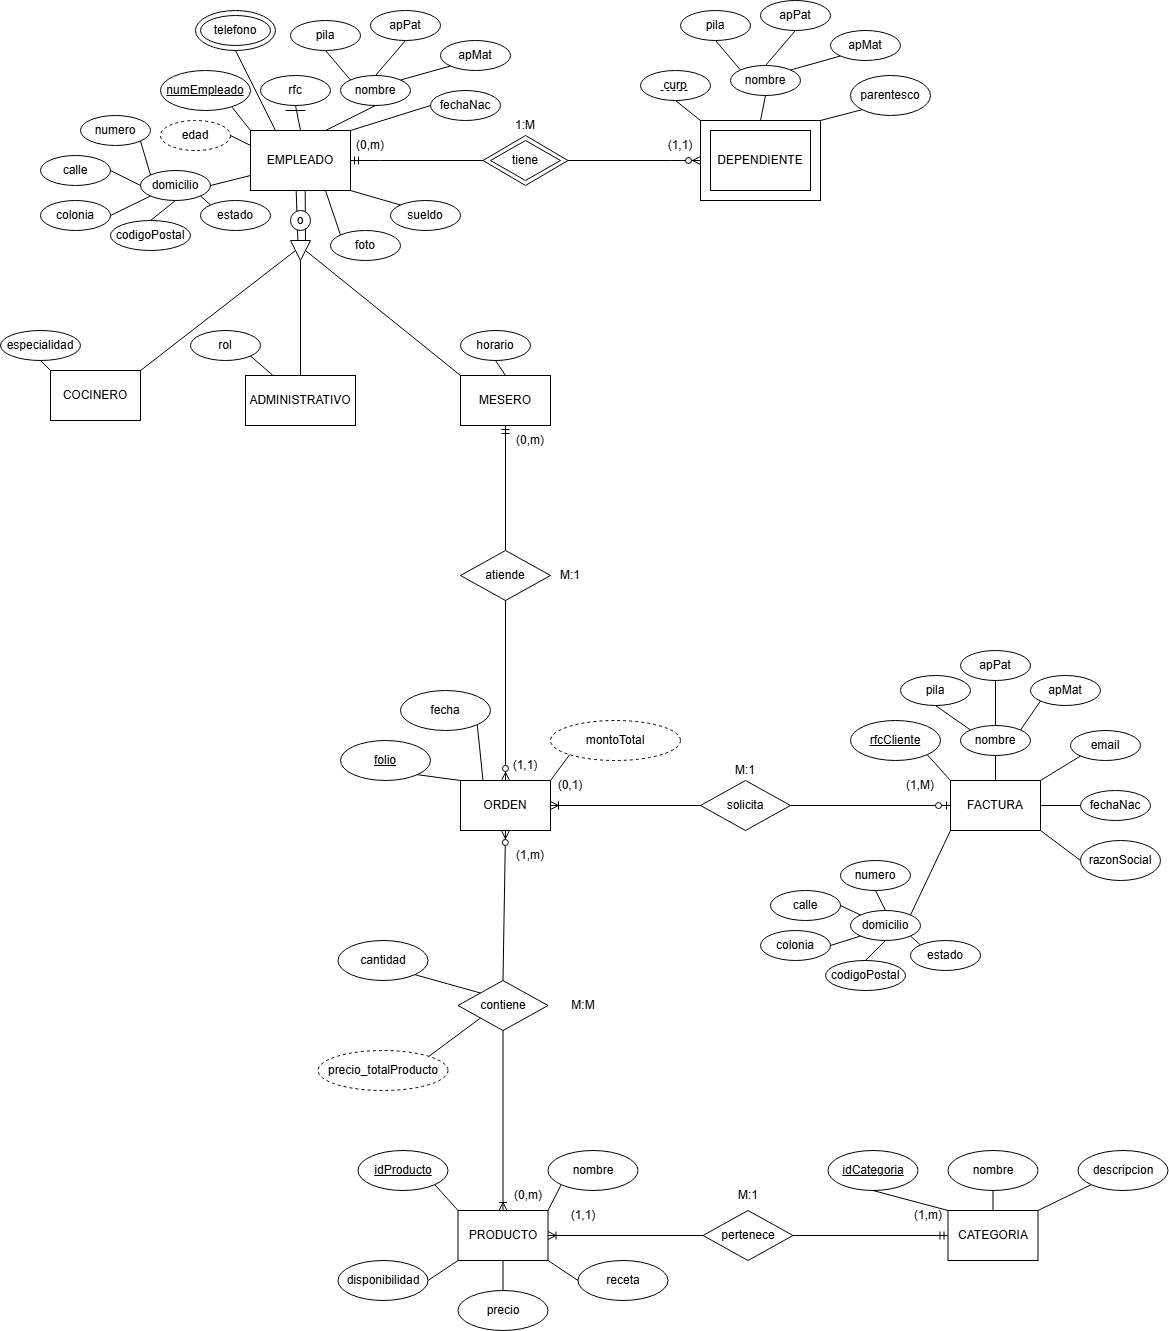
\includegraphics[width=0.95\textwidth]{MER_Restaurante.png}
    \caption{Modelo Entidad-Relación (MER) del sistema de restaurante.}
    \label{fig:mer_restaurante}
\end{figure}

\subsection{Modelo Relacional}
Una vez estructurado el MER, se procedió a realizar el mapeo formal hacia el esquema relacional, aplicando reglas de normalización (hasta la 3FN) para evitar anomalías en las operaciones de inserción, borrado y actualización:
\begin{itemize}
    \item \textbf{Transformación de Entidades y Llaves:} Cada entidad fuerte se convirtió en una relación (tabla) independiente, dotada de una llave primaria (\texttt{PRIMARY KEY}). Se utilizaron secuencias y códigos alfanuméricos 
    como identificadores (por ejemplo, \texttt{folio\_orden} y \texttt{id\_producto}).
    \item \textbf{Resolución de Relaciones $N:M$:} La relación de muchos a muchos entre las órdenes y los platillos se resolvió creando la tabla intermedia (o puente) \texttt{producto\_orden}. Esta tabla almacena las llaves foráneas 
    de ambas entidades y contiene atributos dependientes estrictamente de esa intersección, como la \texttt{cantidad} requerida y el \texttt{precio\_total\_producto}.
    \item \textbf{Integridad Referencial:} Se establecieron restricciones de llave foránea (\texttt{FOREIGN KEY}) para blindar las asociaciones, garantizando que no existan registros "huérfanos". Por ejemplo, el sistema asegura que 
    cualquier factura emitida esté atada a una \texttt{orden} válida, y que toda orden pertenezca a un \texttt{mesero} registrado. \\
\end{itemize}
El diagrama fue realizado en la herramienta \textbf{dbdiagram.io}, por lo que el codigo para generar el diagrama se encuentra en la carpeta del proyecto.
\begin{figure}[H]
    \centering
    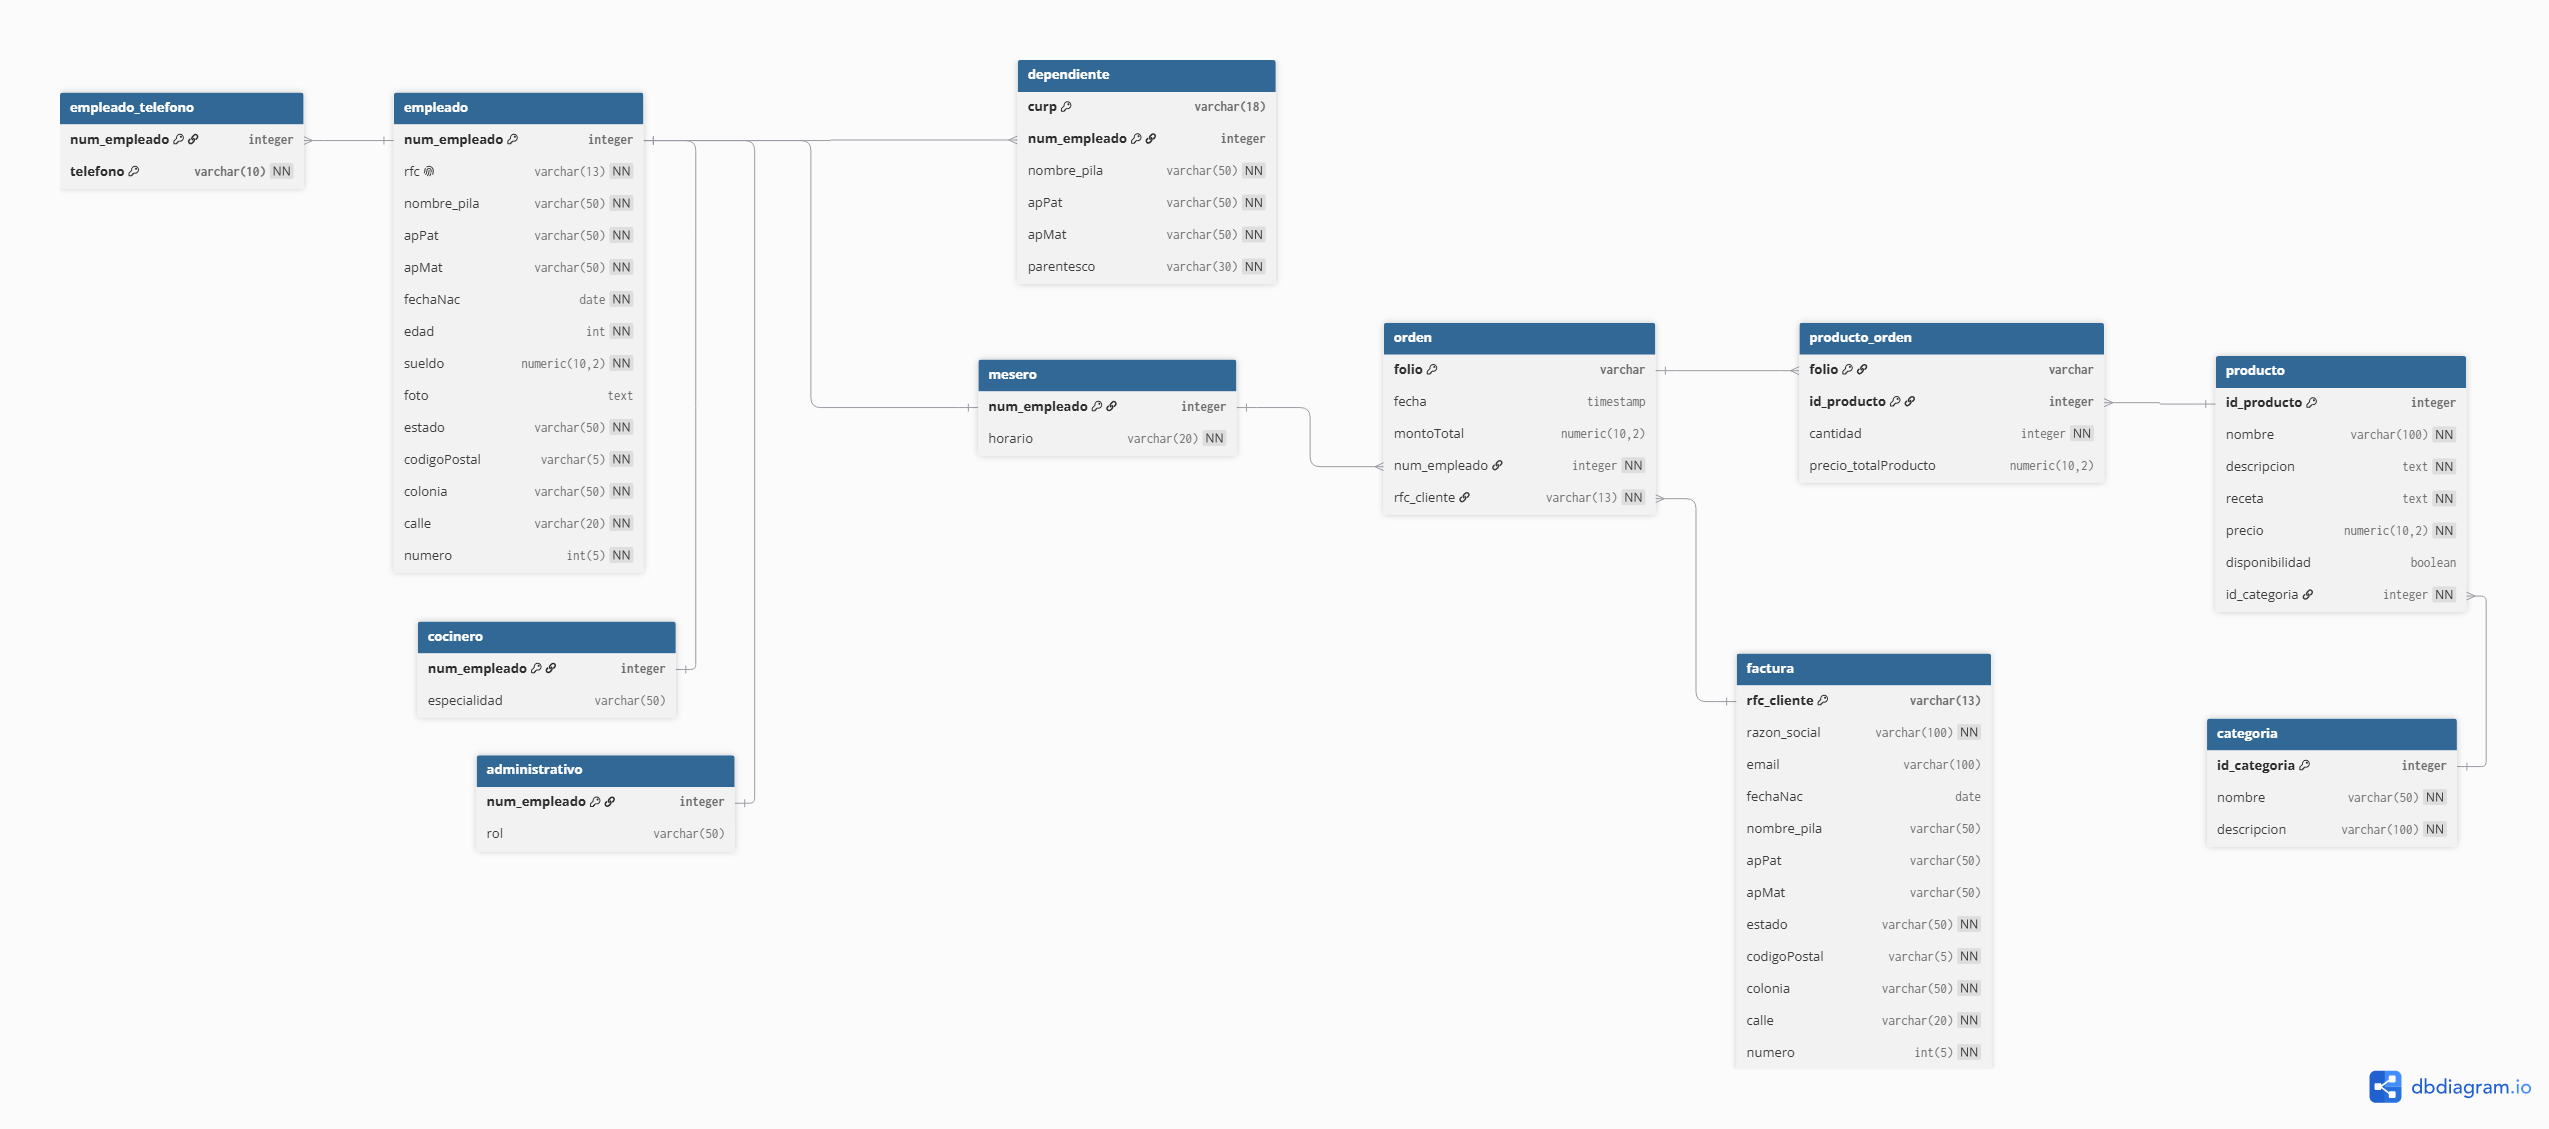
\includegraphics[width=1\textwidth]{MR_Restaurante.png}
    \caption{Modelo Relacional del sistema de restaurante.}
    \label{fig:modelo_relacional_restaurante}
\end{figure}

\section{Implementación}

La base de datos fue materializada utilizando el sistema gestor PostgreSQL. El esquema DDL incluye la creación de tablas con restricciones \texttt{PRIMARY KEY}, \texttt{FOREIGN KEY}, y \texttt{CHECK} para mantener la integridad de dominio.

\textbf{Mecanismos Automatizados Implementados:}
\begin{enumerate}
    \item \textbf{Secuencias Alfanuméricas:} Se implementó una secuencia (\texttt{seq\_folio\_orden}) acoplada a la función \texttt{LPAD} para autogenerar llaves primarias con formato comercial (ej. \texttt{ORD-001}), facilitando el 
    seguimiento visual de los tickets. 
    \begin{figure}[H]
        \centering
        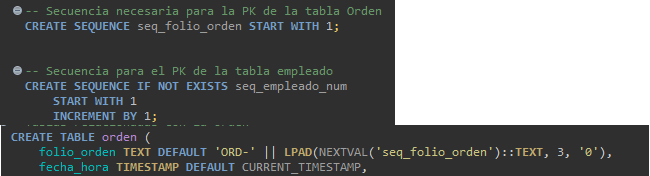
\includegraphics[width=0.5\textwidth]{Implementacion_1.png}
        \caption{Secuencia alfanumérica para generación de folios de orden.}
        \label{fig:secuencia_alfanumerica}
    \end{figure}
    \item \textbf{Trigger 1 - Validación y Subtotales (\texttt{fn\_calcular\_detalle\_orden}):} Este disparador se ejecuta \texttt{BEFORE INSERT OR UPDATE} en la tabla \texttt{producto\_orden}. Su función es consultar la tabla \texttt{producto} 
    para verificar si el platillo tiene la bandera de disponibilidad en \texttt{TRUE}. De ser así, extrae el precio unitario, lo multiplica por la cantidad solicitada y asigna el valor a \texttt{precio\_total\_producto}. Si no está disponible, 
    aborta la transacción lanzando una excepción.
    \begin{figure}[H]
        \centering
        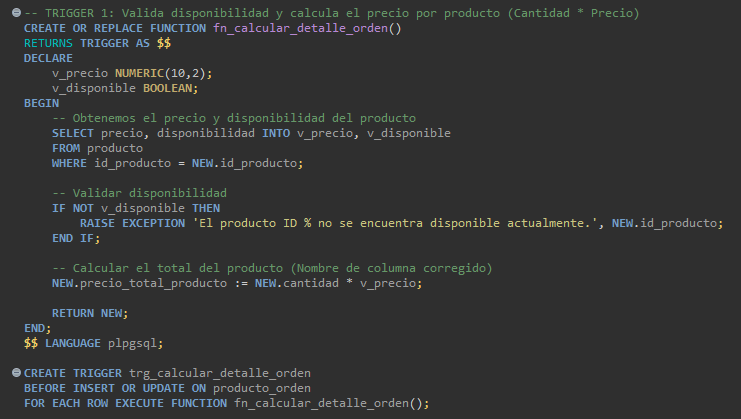
\includegraphics[width=0.5\textwidth]{Implementacion_2.png}
        \caption{Trigger de validación y cálculo de subtotales.}
        \label{fig:trigger_validacion_subtotales}
    \end{figure}
    \item \textbf{Trigger 2 - Actualización de la Orden (\texttt{fn\_actualizar\_total\_orden}):} Se ejecuta tras cualquier cambio en los detalles de la orden. Utiliza la función \texttt{COALESCE} y \texttt{SUM} para recalcular el \texttt{monto\_total} 
    de la tabla \texttt{orden} basándose en todos los productos vinculados a su \texttt{folio\_orden}, garantizando que la cuenta del cliente sea siempre exacta.
    \begin{figure}[H]
        \centering
        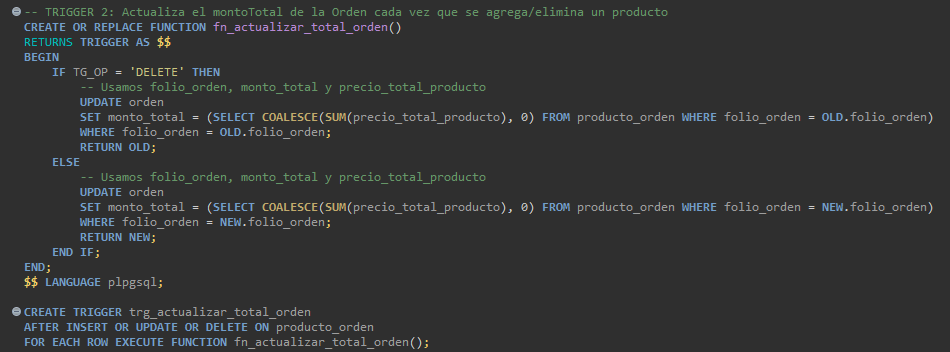
\includegraphics[width=0.5\textwidth]{Implementacion_3.png}
        \caption{Trigger de actualización del monto total de la orden.}
        \label{fig:trigger_actualizacion_orden}
    \end{figure}
\end{enumerate}

\newpage
\section{Presentación}

Para la capa de presentación y conexión hacia la base de datos, se optó por la \textbf{creación de Vistas Estáticas (Views) y Funciones Parametrizadas (Stored Functions) nativas de PostgreSQL}. Esta modalidad permite que cualquier aplicación 
cliente (ya sea un backend o una herramienta de análisis) consuma la información ya procesada, reduciendo la carga de procesamiento en el lado del servidor de aplicaciones.

\textbf{Elementos de Presentación Desarrollados:}
\begin{itemize}
    \item \textbf{Simulador de Factura (\texttt{vw\_factura\_orden}):} Una vista que aplana la complejidad relacional haciendo múltiples \texttt{JOIN}. Concatena domicilios y agrupa los productos consumidos en una sola cadena de texto (\texttt{STRING\_AGG}), 
    entregando un formato tabular listo para ser impreso o exportado a PDF.
    \begin{figure}[H]
        \centering
        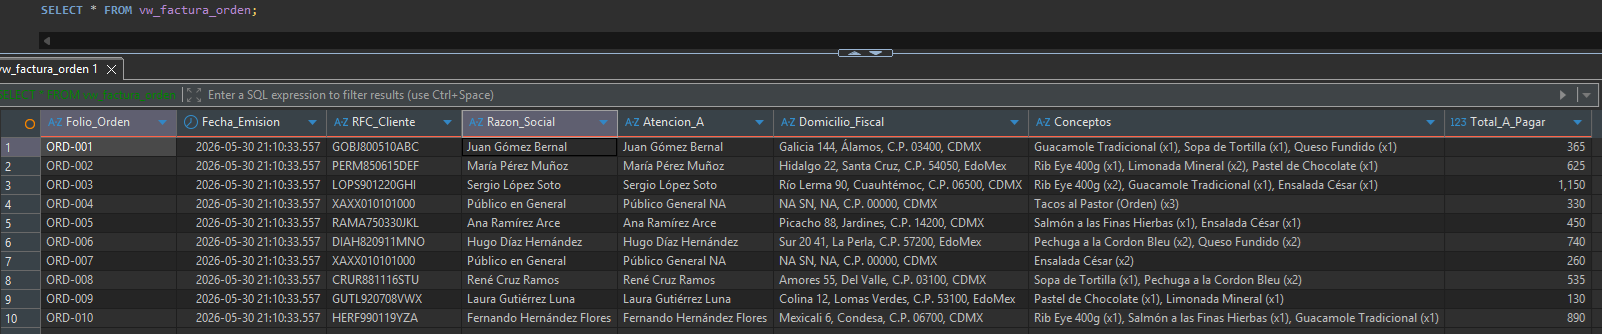
\includegraphics[width=0.95\textwidth]{Presentacion_1.png}
        \caption{Vista para simulación de factura.}
        \label{fig:vista_factura}
    \end{figure}
    \item \textbf{Métricas de Rendimiento (\texttt{fn\_ventas\_por\_periodo} \& \texttt{fn\_rendimiento\_mesero\_hoy}):} Funciones que reciben parámetros de entrada (fechas o ID de empleados) y devuelven tablas resumidas con la cantidad de órdenes 
    atendidas y los montos acumulados, funcionando como un tablero de control gerencial.
    \begin{figure}[H]
        \centering
        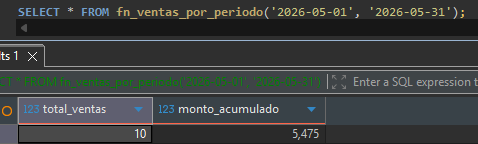
\includegraphics[width=0.95\textwidth]{Presentacion_2.png}
        \caption{Funciones para métricas de rendimiento.}
        \label{fig:funciones_metricas}
    \end{figure}
\end{itemize}

\newpage

\section{Conclusiones}

El desarrollo de este proyecto representó un desafío que me permitió aplicar gran parte de los conocimientos adquiridos a lo largo del curso, los cuales me preparan para enfrentar escenarios reales en la gestión de bases de datos empresariales.

Siendo que uno de los principales retos técnicos durante la etapa de implementación fue la depuración de la lógica interna de PostgreSQL con respecto a la sensibilidad de mayúsculas y minúsculas (camelCase vs. \texttt{snake\_case}). 
Se presentaron errores de sintaxis donde los registros \texttt{NEW} de los triggers no reconocían columnas como \texttt{precio\_total\_producto} debido a inconsistencias de nomenclatura, lo que demandó un proceso riguroso de estandarización en 
todo el código fuente.

Un gran acierto del diseño fue delegar la lógica matemática y las validaciones de negocio directamente al motor de la base de datos mediante Triggers. Esto asegura que, independientemente de la interfaz gráfica o aplicación que inserte los 
datos en el futuro, es imposible registrar un producto agotado o cobrar una orden con cálculos erróneos.  

Este proyecto consolidó mi comprensión sobre la importancia de una correcta normalización y el uso eficiente de secuencias y restricciones. El resultado es un esquema escalable, robusto y preparado para ser el núcleo de un sistema de \
información de nivel empresarial. Además de ayudarme a practicar la identificacion de requerimientos segun el contexto del negocio, lo que es fundamental para cualquier desarrollador de bases de datos.

\end{document}